%% \section{Delta Dictionaries}
\section{Implementation}
\label{sec:DD}

\newcommand{\ddExampleScale}
  %% {0.45}
  {0.50}
  %% {0.55}

\begin{figure}

\centering

%% \begin{figure}[b] %% [H]
\begin{subfigure}[h]{\columnwidth}
  \centering
  \begin{tikzpicture}[nodes = {align = left}]
    \node [scale=\ddExampleScale]
    {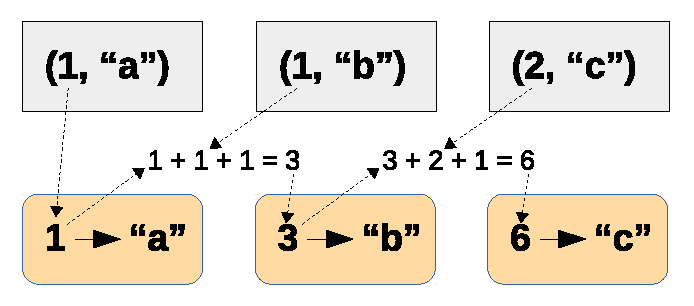
\includegraphics{figs/mech-2-very-short.eps}};
  \end{tikzpicture}
  \caption{An example delta dictionary.}
  %% \caption{What mapping is represented by the \dd~ $\dictP$?}
  \label{fig:dd-example}
\end{subfigure}
%% \end{figure}

\vspace{0.15in}

\begin{figure}[b] %% [H]
  \centering
  \begin{tikzpicture}[nodes = {align = left}]
    \node [scale=.4]
    {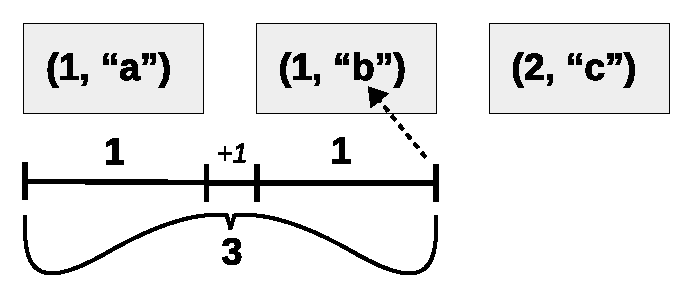
\includegraphics{figs/find-3-very-short.eps}};
  \end{tikzpicture}
  \caption{How do we find key $3$?} %% in the \dd?}
  \label{fig:dd-example-find}
\end{figure}

\vspace{0.15in}

\begin{figure}[H]
  \centering
  \begin{tikzpicture}[nodes = {align = left}]
    \node [scale=.4]
    {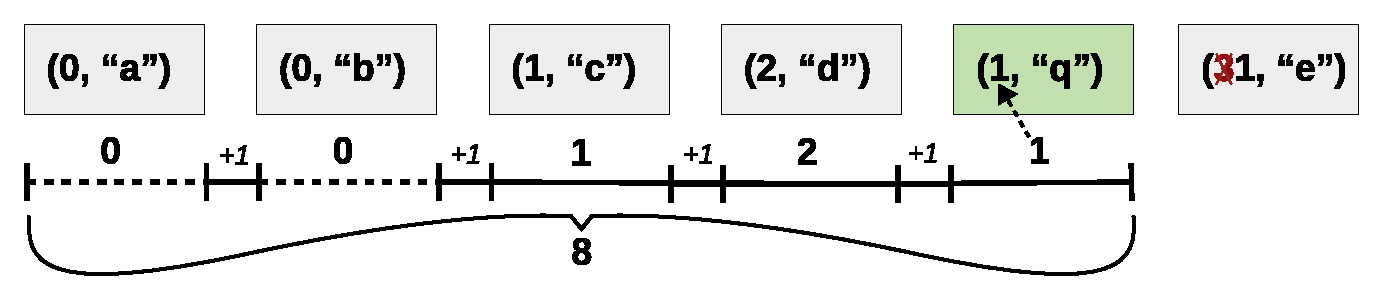
\includegraphics{figs/insert-8.eps}};
  \end{tikzpicture}
  \caption{How do we insert a mapping from key $8$ to value "q"?}
  \label{fig:find-6}
\end{figure}


\caption{Example delta dictionary operations.}
\end{figure}


Our implementation of delta dictionaries and corresponding proofs are formalized in Agda and available in the anonymous supplementary materials.
%
In the paper, we use Haskell, which is simpler and more familiar.

%% \subsection{Delta Indexing}
%% \subsection{Key Types and Deltas}
\subsection{Deltas and Key Types}

Borrowing from association lists, \dds{} use a list-of-pairs, where the first item in each list represents a key and the second is the literal value that is mapped to the represented key.
%
Unlike association lists, the natural number that represents the key is not its literal value.

In order to allow multiple key types, while relying on useful properties of natural numbers under the hood, \dds{} accept a typeclass argument representing a bijection
%
between the key type and the naturals, and use this bijection to convert keys to and from naturals. This is discussed further in \textbf{Bijections to Natural Numbers}.

In order to maintain canonical order, while ensuring that every natural number is valid as the first item in a pair, that number must represent the non-negative difference between the key it represents and the previous key.
%
We call this number a \emph{delta}, alluding to the \emph{delta encoding} technique more commonly harnessed for performance optimization~\citep{XXX}.
%
As described so far, a $0$ offset would correspond to a duplicate key.
%
To prevent duplicate keys from being represented, a delta is actually the offset minus $1$: a delta of $0$ indicates an offset (from the previous key) of $1$, a delta of $2$ indicates an offset of $3$, and so on.
%
The head of the list, however, does not follow the "minus $1$" rule: so the first ``delta'' is interpreted literally, \ie{}~it represents the key value exactly.

\autoref{fig:dd-example} depicts the \dd{} corresponding to the example from \autoref{sec:Introduction}.

%% \subsection{Bijections to the naturals}
%% \label{sec:DD:bij}
\parahead{Bijections to Natural Numbers}

In our implementation, each key is represented by a natural number, so that we can use addition, subtraction, and successor operations in order to define deltas.
%
There may be an algebraic structure more general than the natural numbers which satisfies these requirements, but for practical purposes, working with naturals
%
is easier for both the implementer and the client. In Agda, the bijection typeclass accepts a \texttt{toNat} function, as well as proofs that \texttt{toNat}
%
is injective and surjective, and the \texttt{fromNat} function is defined by the library using the proof of surjectivity. We demonstrate this in Agda by
%
providing an instance of the bijection typeclass for integers ($25$ lines of code).

Most types that are suitable for use as keys in the first place, especially strings and countable numeric types, can be bijected to the naturals,
%
though doing so may be onerous. Finite types, such as characters, are suitable as keys, but cannot be bijected to the naturals -- in these cases,
%
it may be best to harness the theory of finite sets \citep{FinSets}.

\Ddls{} are canonically ordered, but by the natural ordering of the naturals, which, depending on the choice of bijection, may correspond to an unnatural
%
ordering of the key type. As such, we do not expose the ordering to the client -- functions such as \texttt{destruct} and \texttt{toList} return results
%
in arbitrary order, and so from the client's perspective, the \dd{} is unordered.

\subsection{Lookup, Insertion, and Destruction}
\label{sec:DD:basics}

\begin{figure*}
%% TODO using alltt temporarily, to inline DD.hs directly
\begin{alltt}
\input{code/DD.hs}
\end{alltt}
\caption{Delta dictionary implementation in Haskell.}
\label{fig:haskell}
\end{figure*}


\autoref{fig:dd-example-find} and \autoref{fig:dd-example-insert} illustrate example \texttt{lookup} and \texttt{insert} operations.
%
These proceed largely as they would for association lists, but working indirectly with keys encoded as natural numbers and, furthermore, differences between these numbers.

\autoref{fig:haskell} presents concrete implementations for \texttt{lookup}, \texttt{insert}, and \texttt{destruct} in Haskell (rather than Agda) for clarity of presentation.
%
%Having to treat the first delta differently than the rest (literally rather than relatively) is the source of the somewhat technical---through simple---details.

First, we define a helper function \verb+delta+ which computes the delta, \ie{} the offset minus $1$, between two numbers (assuming the second is larger).

Given that, \verb+lookup+ is straightfoward. The \verb+insert+ function is also fairly straightforward - if the first pair is an exact match, then we simply
%
replace the old value with the new one. If the delta to insert is less than delta of the first pair, then we place the delta to insert as the first pair of the new list, and
%
the original first pair will be the second pair of the new list, but using the delta between its original value and the inserted delta.
%
\verb+destruct+ simply pops the head off the list, and then augments the next key by the offset.

%% \cite[Facts about weak maps]{FMapFacts}
%
The Coq Standard \citet[Facts about weak maps]{FMapFacts} lists key metatheory about dictionaries, including that for \verb+lookup+, \verb+insert+, and \verb+destruct+.
%
Our Agda mechanization proves the relevant subset of this metatheory. Some of the metatheory in the Coq treatment involves concepts not relevant to our treatment,
%
especially multiple distinct notions of equality. Also, since we don't expose mapping order to the client via our interface,
%
we do not prove any of the theorems pertaining to ordering (\ie{} those that are not ``weak'').


\subsection{Additional Operations}

Our Agda mechanization also defines key deletion, union, map, and to/from-list operations, along
with appropriate metatheory (not reproduced here).



%% \subsection{Core properties}
%% \section{Properties}
\subsection{Properties}
\label{sec:DD:props}

The \SemInj~ and \EqDec~ theorems, a destruction theorem, and analogs to \emph{contraction} and \emph{exchange} are defined below, and proven in Agda.

%% \subsection{Design Goals}
%% \parahead{Design Goals}

\begin{remark}[\SemTot]
%
\textnormal{This property cannot be formally defined---rather its truth is apparent from the fact that the other theorems do not require their \dd~ arguments to be refined with validity premises.}
%
\end{remark}

\begin{theorem}[\SemInj]
\label{thm:SemInj}

\breakAndIndent
%
For any \dds~ $D_1$ and $D_2$,
%
if for all $k$, $D_1[k] = D_2[k]$,
%
then $D_1 = D_2$.

\end{theorem}

\begin{theorem}[\EqDec]
\label{thm:EqDec}

\breakAndIndent
%
For any \dds~ $D_1$ and $D_2$ whose values are of type $V$,
%
given a function that decides equality for type $V$,
%

\justIndent
%
we can decide that either $D_1 = D_2$ or $D_1 \ne D_2$.

\end{theorem}

%% \begin{theorem}[\EzDstr]
\begin{theorem}[Not-So-Easy Destructibility]
\label{thm:EzDstr}

\breakAndIndent
%
For any \dd~ $D$,

\justIndent \quad
%
either $D = \emptyset$ OR

\justIndent \quad
%
there exist $D'$, $k \notin D'$, and $v$
%
s.t. $D = D' , (k, v)$.

\end{theorem}

%% \subsection{Contraction and Exchange}
%% \parahead{Contraction and Exchange for Dictionaries}

%\rkc{Two common properties for PL metatheory.}

\begin{theorem}[Dictionary Contraction]
\label{thm:cont-dicts}

\breakAndIndent
%
For any {\dd}~ $D$,
%
$D, (k, v'), (k, v) = D, (k, v)$.

\end{theorem}

\begin{theorem}[Dictionary Exchange]
\label{thm:exch-dicts}

\breakAndIndent
%
For any {\dd}~ $D$,
%
if $k_1 \ne k_2$, then
%
$D, (k_1, v_1), (k_2, v_2) = D, (k_2, v_2), (k_1, v_1)$.

\end{theorem}

\parahead{The Difficulty of Destruction}

\SemInj{} requires canonical ordering and deduplication, and \SemTot{} means that the canonical order and deduplication have to come from
how the data is interpreted rather than how it's organized. The non-literal way in which key data is interpreted means that it's not
safe for client code to work with the raw data directly -- rather, all interaction with the data must be
encapsulated in library functions. Unfortunately, this includes \emph{destruction}; an interaction which
normally goes through the very natural, elegant, and well-supported mechanism of pattern matching is now
only available through a library function. The Agda definition of \verb+destruct+ is embellished with proof terms:

\texttt{destruct : (V : Type) (D : dd V) $\rightarrow \\
\phantom{xxxxxxxxxxxxx} D = \emptyset \quad \lor \\
\phantom{xxxxxxxxxxxxx} \exists~(k, v, D')~\left\{~ D = D' , (k, v) \quad \land \quad k \notin D' ~\right\}$}

Just as a list can be destructed with a case expression whose first branch matches nil and whose second branch
decomposes the list into a single item (particularly the head) and the remainder of the list, a \dd~ can be
destructed by matching the result of \verb+destruct+ with a case expression whose left branch handles the
nil dictionary and whose right branch is provided a single item from the dictionary (the mapping $(k, v)$)
and the remainder of the dictionary ($D'$), as well as a proof that $D'$ really is $D$ minus the $(k, v)$
mapping.

This function achieves the same purpose as typical pattern matching (albeit more awkwardly), but because it
doesn't harness the primitive notions of pattern matching and structure, it doesn't establish structural
decrease on the dictionary object, which may break out-of-the-box structural recursion in the likely case
of recursion on $D'$. To enable manual establishment of structural recursion, via an extra parameter that
explicitly tracks the dictionary length, we provide another theorem:

\texttt{dd-extend-length :\\
\phantom{xxxxx} (V : Type) (D : dd V) (k : Key) (v : V) $\rightarrow \\
\phantom{xxxxxxx} k \notin D \rightarrow \\
\phantom{xxxxxxx} |D, (k, v)| = 1 + |D|$}

Although possible, manually establishing termination is painful, especially given that it's not necessary
for {\sal}s or {\cal}s. Thus \dds~ fail at \EzDstr, although they are still better than {\fpf}s in this
regard, seeing as it's not only hard but impossible to destruct {\fpf}s. Is it possible to have a data
structure that possesses all four properties? Not likely - as mentioned above, the combination of
\SemInj~ and \SemTot~ essentially
necessitates that the data in the data structure be interpreted in a non-literal way, which in turn
makes it dangerous for client code to mess with the raw data. As such, we believe we've uncovered an
inherent trade-off between desirable properties. In cases where \EqDec{} is critical,
and the need to destruct dictionaries is occasional but rare, \dds{} seem to be a clear winner over
the conventional solutions. But in cases where dictionaries that don't require \EqDec,
but do require inspection or destruction, {\CAL}s may be a preferable.
